\documentclass[a4paper,12pt]{article}
\usepackage[a4paper,top=3cm,bottom=2cm,left=3cm,right=3cm,marginparwidth=1.75cm]{geometry}
\usepackage[brazil]{babel}
\usepackage[T1]{fontenc}
\usepackage[utf8]{inputenc}
\usepackage{amsmath}
\usepackage{MnSymbol}
\usepackage{wasysym}
\usepackage{hyperref}
\usepackage{color}
\definecolor{Blue}{rgb}{0,0,0.9}
\definecolor{Red}{rgb}{0.9,0,0}
\usepackage{esvect}
\usepackage{graphicx}
\usepackage{float}
\usepackage{indentfirst}
\usepackage{caption}
\usepackage{blkarray}
\newcommand\Mark[1]{\textsuperscript#1}
\usepackage{pgfplots}
\usepackage{amsfonts}
\title{DMDGP: Um Problema Real}
\author{Guilherme Philippi\Mark{*}, orientado por Felipe Delfini Caetano Fidalgo\Mark{\dagger}\\Campus Blumenau\\Universidade Federal de Santa Catarina\\UFSC
\\guilherme.philippi@grad.ufsc.br\Mark{*}, felipe.fidalgo@ufsc.br\Mark{\dagger}}
\begin{document}
	\maketitle
	\tableofcontents
	\newpage
	
	\begin{center}
		\large
		\textbf{Abstract}
	\end{center}
	
	In this paper, two subjects were presented in a disjointed form: The algebra of
	the quaternions and the Problem of Geometry of Molecular Distances. For the first,
	it begins with a historical introduction to quantum algebra and presents some of its	most basic results, monid of its partial or complete demonstrations, as it was found necessary. The same structure forms the second subject, but, due to its nature, a more literary and less formal approach was used. Starting from a contextualisation of the PGDM, some important tools were presented to model it, where, in possession of everything until then, the problem in question can be presented and a brief introduction to the study of its solution.
 
	
	\textbf{Keywords:} Quaternions, MDGP, Distance geometry, Optimization.
	 
	
	\vspace{2cm}	
	\begin{center}
		\large
		\textbf{Resumo}
	\end{center}

	Neste documento foram apresentados dois assuntos de forma disjunta: A álgebra dos quatérnios e o Problema de Geometria de Distâncias Moleculares. Para o primeiro, inicia-se com uma introdução histórica à álgebra de quatérnios e apresenta-se alguns de seus resultados mais básicos, monidos de suas demonstrações parciais ou completas, conforme achou-se necessário. A mesma estruturação forma o segundo assunto, porém, devido a sua natureza, utilizou-se uma abordagem mais literária e menos formal. Partindo de uma contextualização do PGDM, apresentou-se algumas ferramentas importantes para modelá-lo, onde, de posse de tudo até então, pode-se apresentar de fato o problema em questão e uma brevê introdução ao estudo de sua solução. 
	
	\textbf{Palavras-chave:} Quatérnios, PGDM, Geometria de Distâncias, Otimização.
	
	
	\newpage
	\section{Introdução}
	Existe uma relação muito forte com a forma geométrica das moléculas orgânicas e suas funções em organismos vivos. Pode-se fazer uma analogia destes organismos com um grande quebra-cabeça, cheio de peças tão variadas quanto se queira, onde cada peça tem um local específico no grande quebra-cabeça, de forma que sua posição e função é dado justamente pela forma geométrica de cada peça. Imagine este grande quebra-cabeça de forma tridimensional ao invés de plana, com peças em formatos diversos e escalafobéticos, logo, você não estará tão longe de entender como funciona um organismo vivo.
	
	Outrora, em pesquisas sobre a molécula de DNA (ácido desoxirribonucleico), descobriu-se que essa era parte fundamental da produção de um dos pilares para a vida: a proteína. Esta será o alvo principal deste estudo e possuí uma gama extensa de funções em nosso organismo --- como se fossem as tais peças do quebra-cabeça da analogia acima. Podemos dizer que somos feitos de proteínas. Organismos vivos lutam constantemente contra a desorganização intrínseca do universo e as proteínas tem papel importantíssimo nessa luta. São elas as estruturas que utilizamos para nos organizar, gerando informação, ao possibilitarem um mecanismo procedural natural para a vida, como com o seu papel no transporte de oxigênio (hemoglobina), na proteção do corpo contra organismos patogênicos (imunoglobulina), com a catalização de reações químicas (apoenzima), além de outras inúmeras funções primordiais no nosso organismo \cite{fidalgotese}. Perceba a importância fundamental em estudar a estrutura geométrica de cada uma dessas proteínas e sua relação com suas funções.
	
	Por conta dessa motivação tem-se esforços como o de Kurt Wüthrich, que propôs que se utilizasse experimentos de \textit{Ressonância Magnética Nuclear}
	(RMN) para calcular a estrutura tridimensional de uma molécula de proteína, ganhando o premio Nobel da Química em 2002 \cite{RMNproteinWrutrich}. Porém, a partir dessa estratégia tivemos novos problemas. A RMN não tem como resultado a estrutura tridimensional de uma proteína, mas sim distâncias entre átomos relativamente próximos que compõem a proteína. Para poder calcular a estrutura de uma proteína a partir dessas distâncias, surgira um novo problema, conhecido na literatura como \textit{Problema de Geometria de Distâncias Moleculares}, ou simplesmente, MDGP \cite{carlileGDandAplications}.
	
	Ao longo desse texto estudaremos este problema, suas variações, seus problemas relacionados, as ferramentas que nos facilitarão a resolve-los, suas soluções e as complexidades relacionadas a estas soluções.
	
	\newpage

	\section{Materiais e Métodos}
	
	\newpage
	
	\section{Grafos: Aspectos Gerais}
	
	\newpage
	
	\section{Um Passeio pela Bioquímica}
	A bioquímica é a ciência que busca explicar as formas e funções biológicas em termos químicos, uma tarefa muito divertida, porém, complicada. Já no século XVIII, os químicos percebiam a grande diferença entre o mundo inanimado e o mundo vivo: Antoine-Laurent Lavoisier (1743-1794) constatou a relativa simplicidade do ``mundo mineral'' --- não orgânico --- comparada a complexidade dos ``mundos animal e vegetal'' \cite{bioquimicaLehninger}. Ele sabia que esses últimos eram constituídos de moléculas ricas nos elementos carbono, oxigênio, nitrogênio e fósforo, que, devido sua abundância na natureza somada com as suas características químicas, são ótimos para constituírem a complexidade da vida.

	\subsection{Carbono}
	A química dos organismos vivos está organizada em torno do carbono, pois este é muito comum na natureza e possuí uma ótima propriedade estrutural: O carbono pode formar ligações simples estáveis com até quatro outros átomos. De fato, o carbono constitui mais da metade do peso seco das células. 
	
	Sabe-se, através de experimentos de cristalografia \cite{ramachandran1974MolStructure}, muito sobre a geometria das ligações dos átomos de uma proteína. Em particular, as quatro ligações simples do carbono formam um tetraedro (vide Figura ~\ref{fig:carbono}, retirada de \cite{bioquimicaLehninger}) com ângulos de 109,5\textdegree entre duas ligações quaisquer e comprimento médio de ligação de 1,54\AA\footnote[1]{Unidade física para distâncias atômicas é o Ângstron (\AA), onde equivale a 1\AA = $10^{-10}$ m.}. Existe também uma outra característica muito importante para nós nas ligações do carbono: Sabe-se que as ligações simples podem rotacionar livremente (a menos que grupos muito grandes ou altamente carregados estejam ligados aos átomos de carbono, onde, neste caso --- e, na verdade, esse é o caso comum ---, a rotação é regida pelo equilíbrio de forças na molécula \cite{carlileTese}, que pode ser limitada), enquanto que as ligações duplas são mais curtas (em torno de 1,34\AA) e não permitem rotação. Perceba também o plano formado pelos átomos A, B, X e Y na Figura ~\ref{fig:carbono}.

	\begin{figure}[H]
		\begin{center}
			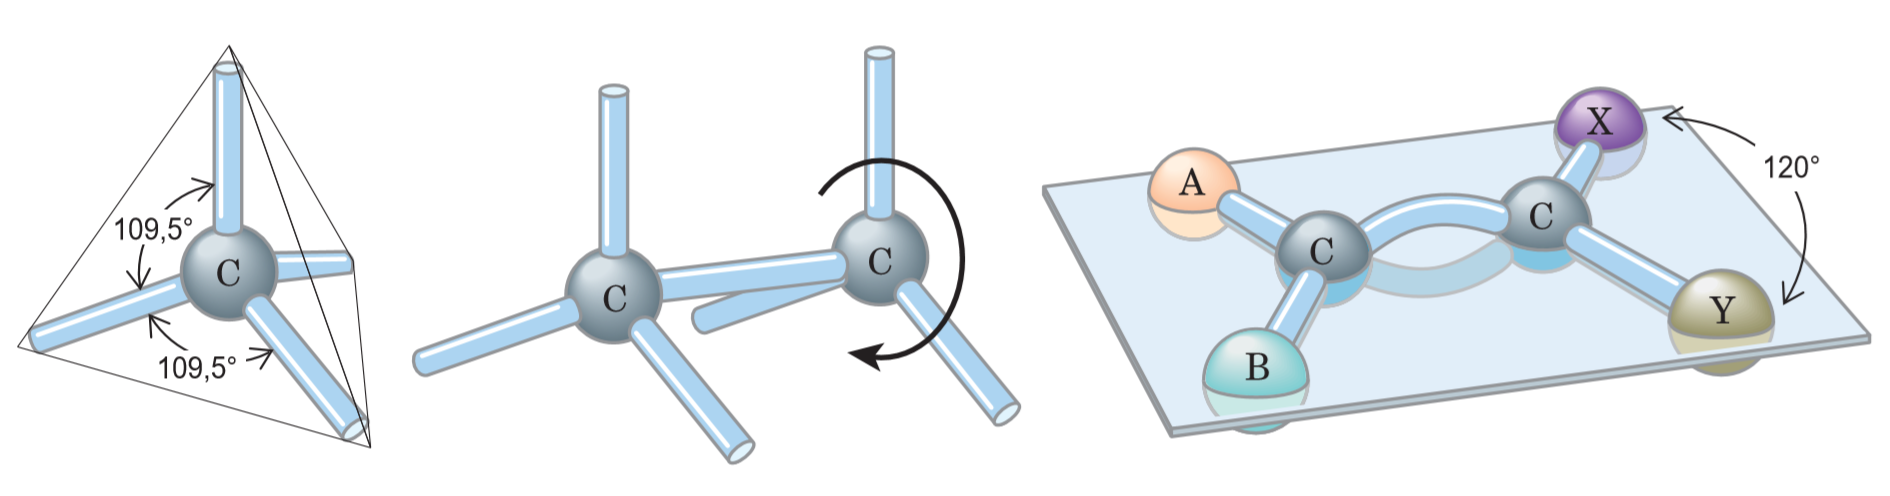
\includegraphics[width=1\linewidth]{carbono.png}
		\end{center}
		\caption{Geometria da ligação do carbono.}
		\label{fig:carbono}
	\end{figure}

	A versatilidade das ligações covalentes do carbono podem formar cadeias lineares, ramificadas e estruturas cíclicas. Nenhum outro elemento químico consegue formar moléculas com tanta diversidade de tamanhos, formas e composição.
	
	\subsection{Classificação Macromolecular}
	As células contém um conjunto universal de moléculas pequenas. Mas como podemos discutir sobre o que é uma molécula pequena, média ou grande? Devemos definir uma forma de comparar os tamanhos moleculares. Na literatura existem duas medidas principais para esse fim, com uma relação bem definida entre si	, tratam-se do \textit{peso molecular} --- ou \textit{massa molecular relativa} ---, denominado $M_r$ e da \textit{massa molecular}, denotada simplesmente por $m$. O peso molecular é definido como uma relação direta da massa da molécula da substância estudada com um duodécimo da massa do carbono-12 ($^{12}C$, em torno de $1,9926\times 10^{-23}$ gramas), note que, como $M_r$ é uma razão, não possui dimensão associada. Já a massa molecular é apenas a massa da molécula (ou massa molar) sobre o número de Avogadro --- que é definida como sendo o número de átomos por mol de uma determinada substância.
	
	
	
	Ao se estudar proteínas, logo se percebe sua imensidão, tanto em número como em diferenças, porém, algumas características se mantem em comum entre elas. Sabe-se que todas são formadas por aminoácidos, visto que apenas eles restam quando uma se degrada. Existem vinte tipos de aminoácidos naturais e da combinação destes por ligações petídicas formam-se todas as proteínas conhecidas. \cite{fidalgotese}
	
	Destes vinte aminoácidos, dezenove tem uma estrutura básica em comum, um carbono principal (ou também chamado, carbono alfa) ligado a um grupo amina e um grupo carboxílico. O que diferencia esses dezenove aminoácidos é o radical (ou grupo variável). Na ilustração abaixo os radicais são representados por $R_1$ e $R_2$.
	\\
	\begin{figure}[H]
		\begin{center}
			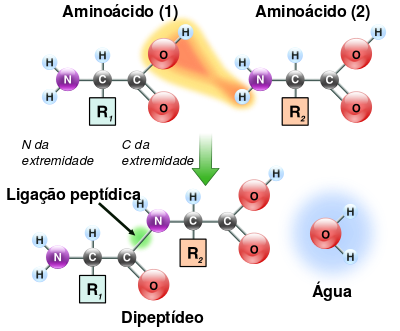
\includegraphics[width=0.6\linewidth]{Peptidformation.png}
		\end{center}
		\caption{Estrutura de um aminoácido e a síntese proteica}
		\label{}
	\end{figure}
	
	Por tanto, há uma noção prévia de qual tipo de estrutura esperar ao analisar uma molécula de proteína, isto é, existe uma ordem conhecida para as ligações dos átomos. Como as ligações atômicas vêm de processos físico-químicos, há na literatura a distância e ângulo associados a cada tipo diferente de ligação e pares de átomo. Neste problema trataremos apenas de ligações covalentes, pois há o compartilhamento de elétrons.
	
	\subsection{wwPDB}
	
	\newpage
	\section{\textit{Molecular Distance Geometry Problem}}
	
	\subsection{Geometria de Distâncias}
	O principal conteúdo de estudo da Geometria de Distâncias, como o próprio nome sugere, rodeia a ideia de distância entre objetos de determinada estrutura geométrica. Assim, o problema fundamental da Geometria de Distâncias consiste em determinar um conjunto de pontos, pertencentes a um espaço geométrico, com base nas distâncias conhecidas entre tais pontos. Note que nem sempre sabemos todas as distâncias entre todos os pontos.
	\subsubsection*{Breve Histórico sobre Geometria de Distâncias}
	Temos que o surgimento da Geometria de Distâncias deu-se por volta de 1928, com o matemático Karl Menger. Entretanto, somente em 1953, com Leonard Blumenthal, que a Geometria de Distâncias tornou-se uma nova área de conhecimento.
	\\
	Por outro lado, somente em 1978, com Yemini, que o problema fundamental de Geometria de Distâncias foi enunciado. Problema onde não sabemos todas as distâncias.
	\\
	Em 1988, temos o início da utilização da Geometria de Distâncias para o cálculo de Proteínas.
	
	\subsection{Representações dos Átomos em Coordenadas\label{sec:bi}}
	Como as partículas que estamos interessados estão localizadas no espaço tridimensional, podemos representa-las utilizando coordenadas cartesianas tridimensionais $x_1, ...,x_n \in\mathbb{R}^3$, onde $x_n$ é a \textit{realização} do n-ésimo átomo da molécula analisada. 
	
	Além da utilização das coordenadas cartesianas, também se faz uso de outro sistema de coordenadas, mais condizente com os dados que se tem a priori da molécula, antes da solução do problema. Tal sistema denomina-se \textit{coordenadas internas}.
	
	As coordenadas internas de uma proteína são definidas pela distância entre os átomos $d_{1,2}, ..., d_{n - 1,n}$, pelo ângulo planar $\theta_{1,3}, ...,\theta_{n - 2,n}$ (formados por 3 átomos consecutivos) e pelos ângulos de torção $\omega_{1,4}, ..., \omega_{n-3,n}$ (formado por 4 átomos consecutivos). O ângulo de torção é o ângulo entre os planos formados pelos átomos $i-3,i-2,i-1$ e$i-2,i-1,i$, respectivamente. Assim, temos que $\omega$ varia no intervalo $[0,2\pi]$ e $\theta$ de $[0,\pi]$, assim como em um sistema de coordenadas esféricas, e também sabe-se da literatura que as distâncias entre os átomos unidos por ligações covalentes é em torno de 1,5\AA. Em vista desta curta distância típica, convenciona-se selecionar apenas pares de átomos tais que $d_{i,j}\leq 5 $\AA 
	\\
	
	\begin{figure}[H]
		\begin{center}
			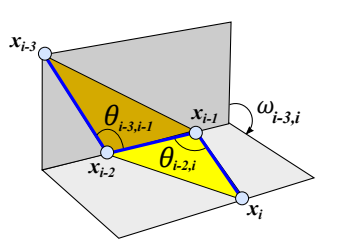
\includegraphics[width=0.6\linewidth]{Capturar.PNG}
		\end{center}
		\caption{Ângulos planos e de torção}
		\label{fig:angulos}
	\end{figure}
	
	Pode-se obter facilmente os ângulos planos pela \textit{Lei dos Cossenos}, tendo em vista que conhece-se todas as distâncias que, por construção, representam os lados do triângulo. Também não se encontra dificuldades para determinar os ângulos de torção, podendo utilizar da \textit{Geometria Analítica} para descobrir o ângulo entre dois vetores. Para mais detalhes, recorrer ao Apêndice A.
	
	Como trabalharemos com valores associados às distâncias entre átomos, é claramente notável a importância de se determinar as coordenadas cartesianas a partir das coordenadas internas. Para isso, utiliza-se uma série de operações que estão descritas pelas matrizes abaixo.
	
	Consideremos que as coordenadas do ponto $x_{i} \in\mathbb{R}^3,i= 1, ...,n $ são dadas por $(x_{i1},x_{i2},x_{i3})$, temos:
	
	$$
	\begin{bmatrix}
	x_{i1}\\ 
	x_{i2}\\ 
	x_{i3}\\ 
	1
	\end{bmatrix}
	= B_{1}B_{2}\cdots B_{i}\begin{bmatrix}
	0\\ 
	0\\ 
	0\\ 
	1
	\end{bmatrix},
	$$
	onde
	$$
	B_1\: =\:
	\begin{bmatrix}
	1 & 0 & 0 & 0\\ 
	0 & 1 & 0 & 0\\ 
	0 & 0 & 1 & 0\\ 
	0 & 0 & 0 & 1
	\end{bmatrix},\:\:\:
	\: B_2\: =\:
	\begin{bmatrix}
	-1 & 0 & 0 & -d_{1,2}\\
	0 & 1 & 0 & 0\\ 
	0 & 0 & -1 & 0\\ 
	0 & 0 & 0 & 1
	\end{bmatrix},
	$$
	$$
	B_3\:=\:
	\begin{bmatrix}
	-\cos\theta_{1,3} & -\sin\theta_{1,3} & 0 & -d_{2,3}\cos\theta_{1,3}\\ 
	\sin\theta_{1,3} & -\cos\theta_{1,3} & 0 & d_{2,3}\sin\theta_{1,3}\\ 
	0 & 0 & 1 & 0\\ 
	0 & 0 & 0 & 1
	\end{bmatrix}
	$$
	e
	$$
	B_i\:=\:
	\begin{bmatrix}
	-c_{\theta_{i}} & -s_{\theta_{i}} & 0 & -d_{i-1,i}c_{\theta_{i}}\\ 
	s_{\theta_{i}}c_{\omega_{i}} & -c_{\theta_{i}}c_{\omega_{i}}
	& -s_{\omega_{i}} & d_{i-1,i}s_{\theta_{i}}c_{\omega_{i}}\\ 
	s_{\theta_{i}}s_{\omega_{i}} & -c_{\theta_{i}}s_{\omega_{i}} & c_{\omega_{i}} & d_{i-1,i}s_{\theta_{i}}s_{\omega_{i}}\\ 
	0 & 0 & 0 & 1
	\end{bmatrix}
	$$
	onde $s_{\theta_{i}}=\sin (\theta_{i-2, i}),\: c_{\theta_{i}}=\cos (\theta_{i-2, i}),\: s_{\omega_{i}}=\sin (\omega_{i-3, i}),\: c_{\omega_{i}}=\cos (\omega_{i-3, i})$. Em $B_i$, $i=4, ..., n$.
	
	
	Perceba que $B_i$ é a matriz que engloba todas as operações necessárias para encontrar a i-ésima realização do i-ésimo átomo da molécula tendo conhecimento de todas as matrizes $B_j$ $\forall j < i$. Como é de grande importância o entendimento de tais operações que formam a $B_i$, deixa-se o Apêndice B para esta discussão.
	
	Note também que fixando-se os comprimentos das ligações covalentes $d_{1,2},d_{2,3}$ e o valor do ângulo plano $\theta_{1,3}$, os três primeiros átomos terão as coordenadas dadas por
	$$
	x_1\:=\:
	\begin{bmatrix}
	0\\ 
	0\\  
	0
	\end{bmatrix},\:\:\:
	x_2\:=\:
	\begin{bmatrix}
	-d_{1,2}\\ 
	0\\  
	0
	\end{bmatrix},\:\:\:
	x_3\:=\:
	\begin{bmatrix}
	-d_{1,2}+d_{2,3}\cos\theta_{1,3}\\ 
	d_{2,3}\sin\theta_{1,3}\\  
	0
	\end{bmatrix}
	$$
	
	Podemos observar que dados estas três realizações dos três primeiros átomos fixamos a base do sistema, evitando estruturas obtidas por meio de rotações e translações a partir de uma mesma estrutura.	
	
	\subsection{Ressonância Magnética Nuclear}
	A ressonância magnética nuclear é um processo físico que analisa a interação da radiação eletromagnética com a matéria. Neste experimento é escolhida uma faixa de radiofrequência para bombardear uma amostra que está imersa em um campo magnético bastante intenso. Dependendo da radiofrequência utilizada, alguns núcleos atômicos irão absorver energia e outros não. Caso atinja-se uma frequência exata de ressonância dentro destes núcleos atômicos, é possível medir essa ressonância como um sinal de radiofrequência enviado dos núcleos atômicos. No PGDM, a frequência utilizada é para a ressonância dos núcleos de hidrogênio e um computador capta essas respostas eletromagnéticas dos núcleos atômicos para utilizar como dados do problema. \cite{RMNBookIntroduction}
	
	Assim, esse procedimento fornece vários \textit{intervalos} de distâncias possíveis relativas associadas a átomos de hidrogênio próximos (sendo que por vezes também 
	é capaz de captar átomos de um isótopo específico de carbono, devido a proximidade de sua frequência com a do hidrogênio), esses intervalos também são chamados de \textit{distancias intervalares}. Pode-se representar essas distancias intervalares matematicamente por intervalos de números reais $[d_{i,j}^i, d_{i,j}^f]$ . Isto é, existe um real $d_{i,j}$ que representa a distância real tal que
	
	$$ 0 \leq d_{i,j}^i \leq d_{i,j} \leq d_{i,j}^f$$
	
	\subsection{Modelagem Matemática}
	Quando um cientista de outra área se depara com um problema que não consegue resolver e precisa recorrer aos matemáticos, quase sempre se torna uma tarefa muito complicada para quem for tentar desenvolver o problema. Não pela complexidade matemática do assunto, isto os matemáticos dominam. A dificuldade está em entender o problema de outras áreas e, como se por ironia, resolve-los. Este é um fardo que se tem de carregar quando se escolhe trabalhar com uma ciência que é utilizada por tantas outras. No entanto, por sorte, os matemáticos são apaixonados por interpretar, modelar e resolver problemas.
	
	A boa interpretação de um problema de matemática aplicada deve se ater a algumas perguntas importantes:
	\begin{itemize}
		\item \textbf{Quais são as hipóteses?} Ou seja, fatos dos quais devemos nos basear e nos limitar para propor, de forma dialética, uma solução para o problema. Nos importaremos com seis hipóteses que advém de informações já discutidas aqui:
		\begin{description}
			\item[Hipótese 1:]as distâncias fornecidas pelos experimentos de RMN estão associados a pares de átomos conhecidos: nós sabemos a quais átomos as distâncias se referem (isso não é bem verdade, mas supomos que seja assim para desenvolver o problema);
			\item[Hipótese 2:]todos os átomos da molécula da proteína cuja estrutura 3D queremos calcular são conhecidos: conhecermos a estrutura química da molécula;
			\item[Hipótese 3:]todos os átomos da molécula de proteína estão ligadas a algum átomo, cuja distância é conhecida: não há átomos soltos, afinal, se existisse, seria outra molécula;
			\item[Hipótese 4:]existe uma ordem, dada a priori, entres os átomos da cadeia principal da proteína cuja estrutura 3D queremos calcular: conhecemos o esqueleto padrão, formado de aminoácidos, da molécula de proteína examinada;
			\item[Hipótese 5:]as distâncias entre os átomos de uma molécula de proteína separados por duas ligações covalentes são conhecidas: existem esses resultados na literatura;
			\item[Hipótese 6:]as distâncias fornecidas pela RMN são representandos por intervalos de números reais que contêm o valor correto associado.
		\end{description}
		
		\item \textbf{Qual resultado deseja-se obter?} De forma simplificada, qual é nossa \textit{tese}? Dificilmente se chega no lugar ideal se não há o conhecimento da direção a seguir. Cabe-se uma definição formal dos nossos objetivos:
		
		\textit{Deve-se determinar os pontos} $x_{i}\in\mathbb{R}^3$, \textit{i = 1, ..., n (n é o número de átomos da molécula), satisfazendo as equações}
		$$\|x_i -x_j\|=d_ij , \forall\in E
		$$
		\textit{onde} $E \subset \{1, ...,n\} \times \{1, ...,n\}$ e $d_{ij}$ \textit{são os valores de distâncias fornecidas pela RMN.}
		
		Tentar resolver os sistemas de equações acima parece não ser uma boa ideia, já que existem evidências de que não seja possível obter uma fórmula fechada para isso \cite{carlileBook31Coloquio}. Podemos até tentar resolver numericamente, porém as soluções seriam infinitas para as equações.
		
		A abordagem mais usual é a representação do problema usando otimização. Para isso devemos  resolver todas as equações do problema. Podemos, dessa maneira, considerar uma única expressão com todas elas, dada por
		$$ f(x_1, ...,x_n) \equal \sum_{(i,j) \in E} (\|x_i - x_j\| - d_{ij})^2
		$$
		
		Para resolvermos tal otimização, basta encontrar valores de $x_i \in \mathbb{R}^3$, $i = 1, ..., n$, tal que $f(x_1, ...,x_n)=0.$ Assim temos
		$$ \min_{x_t \in\mathbb{R}^n} f(x_1, ...,x_n).
		$$
		
		A dificuldade nesse caso está em encontrar o mínimo global, pois existem vários mínimos locais e estes\textit{ crescem exponencialmente com a  quantidade de átomos da molécula}. Outro ponto delicado, é complicado distinguir mínimo local de global, uma vez que os métodos de otimização continua só se referem a informações locais. Isso tudo torna o problema muito custoso para resolver.
	\end{itemize}
	
	\subsubsection*{Problema de Geometria de Distâncias Moleculares: Uma definição formal}
	Agora que temos uma boa base, vamos definir o Problema de Geometria de Distâncias Moleculares formalmente utilizando grafos.
	\\
	
	Dado um grafo simples não-direcionado $G=(V,E)$, de modo que suas arestas sejam valoradas por uma função não-negativa $d:E\rightarrow\mathbb{R_+}$, considere a seguinte aplicação:
	$$x:V\rightarrow\mathbb{R}^3
	$$
	De modo que para todo $\{u,v\}\in E$ temos:
	$$\|x(u)-x(v)\|=d({u,v})
	$$
	Logo, nossa tarefa é encontrar uma aplicação $x$ que satisfaça todas as distâncias e dados do grafo que temos. Esta função é denominada \textit{realização} de $G$. Quando a realização satisfaz todas as equações da forma "$\|x(u)-x(v)\|=d({u,v})$", dizemos que ela é uma \textit{realização válida}.
	
	
	\subsection{Modelagem Computacional}
	
	Uma vez que existe uma introdução a modelagem matemática do problema, pode-se pensar em uma abordagem computacional. Não é segredo para ninguém que a computação veio e vem melhorando muito a forma como se faz matemática, introduzindo novas ferramentas e campus de estudo de grande importância. Vamos utilizar dessa evolução para a solução desse problema que, de outra forma, não seria viável. Na verdade, um dos estudos que estamos despostos a fazer aqui é se, mesmo com toda nossa capacidade computacional atual, o problema tem uma solução viável. Definiremos melhor adiante o que é uma solução dita \textit{viável}. 
	
	\subsubsection*{Dados de Entrada e Saída}
	É costume de programação se preocupar em deixar claro quais dados devem ser de entrada (\textit{input}), para serem utilizados, processados, modificados e todo o resto que necessitar para gerar os dados de saída (\textit{output}).
	
	Existem dois tipos de dados que serão tratados aqui, os dados \textit{teóricos} e os dados \textit{reais}. Todos os dados reais que utilizamos são provenientes dos experimentos de RMN. Já os teóricos vem de conhecimento da Química, Física e Biologia.
	
	\begin{description}
		\item{Dados de Entrada:}
		\begin{itemize}
			\item quantidade de átomos: $n$;
			\item sequências de átomos:
			$$N^1,C^{1}_{\alpha},C^1,N^2,C^{2}_{\alpha},C^2, ...,N^{n/3},C^{n/3}_{\alpha},C^{n/3};
			$$
			\item distância entre os átomos separados por uma ligação covalente: $\{d_{1,2},d_{2,3}, ...,d_{n-1,n}\}$, onde $i = 2, ..., n;$
			\item distância entre os átomos separados por duas ligações covalentes: $\{d_{1,3},d_{2,4}, ...,d_{n-2,n}\}$, $i=3, ..., n;$
			\item distância entre átomos próximos, com no máximo 5 \AA, fornecidas pela RMN \textit{- único dado de entrada real};
		\end{itemize}
		\item{Dados de Saída:}
		\begin{itemize}
			\item posições $x_1, ...,x_n \in\mathbb{R}^3$ dos $n$ átomos da proteína.
		\end{itemize}
	\end{description}
	
	Como as distâncias fornecidas pela RMN são um dado real, não são um valor exato. Dados reais são incertos, dependem de muitas variáveis, como a precisão da ferramenta que a mediu, o tipo de medida, quantas vezes fora medido, entre outras coisas. Esta incerteza é calculada e pode-se saber mais sobre em \cite{EstatisticaTratamentoDeDados}.
	
	\subsubsection*{Complexidade do PGDM}
	É de extrema importância verificarmos o curso computacional de se tentar resolver o PGDM, pois, só com esta analise, pode-se dizer se o problema tem ou não uma solução viável. Caso não tenha, o trabalho pode ser encerrado por aqui. De nada nos adianta solução que não pode ser calculada.
	
	Para poder calcular o custo computacional de uma solução matemática, deve-se verificar quantas vezes o \textit{núcleo} do programa é computado, ou seja, se verifica quantas vezes a operação central do programa é realizada. Caso for realizada apernas uma vez, dizemos que o custo é baixo. Caso essa quantidade cressa proporcionalmente a medida que aumentamos os dados de entrada do problema (por exemplo, a medida que aumentamos a quantidade $n$ de átomos da molécula), então dizemos que a dificuldade é linear. Para mais detalhes sobre custo computacional, leia \cite{ComplexidadeComp}. Resolvemos, então, um PGDM simples e verificamos qual seria seu custo.
	
	Considere um PGDM restrito ao plano, onde temos um grafo $G = (V(G), E(G))$ tal que $V(G)=\{u, v, r, s\}$ e $E(G)=\{\{u,v\}, \{u, r\}, \{v, r\}, \{v, s\}, \{r, s\}, \{u, s\}\}$. Fixando \textit{u, v, r} e \textit{s}, ou seja, determinando $ x_{u}, x_{v},x_{r} \in\mathbb{R}^2$ de tal modo que $\|x_{u} - x_{v}\|= d_{uv}$,  $\|x_{u} - x_{r}\|= d_{ur}$ e $\|x_{v} - x_{r}\|= d_{vr}$, podemos montar o  seguinte sistema quadrático:
	$$ \|x_{s} - x_{u}\|= d_{us} $$$$ \|x_{s} - x_{v}\|= d_{vs} $$$$ \|x_{s} - x_{r}\|= d_{rs} $$
	Elevando os termos ao quadrado,
	$$\|x_{s}\|^{2} - 2(x_{s}.x_{u}) + \|x_{u}\|^{2} = d_{us}^{2}$$
	$$\|x_{s}\|^{2} - 2(x_{s}.x_{v}) + \|x_{v}\|^{2} = d_{vs}^{2}$$
	$$\|x_{s}\|^{2} - 2(x_{s}.x_{r}) + \|x_{r}\|^{2} = d_{rs}^{2}$$
	subtraindo a primeira equação das outras duas, temos:
	$$2(x_{s}.x_{v}) - 2(x_{s}.x_{u}) = \|x_{v}\|^{2} - \|x_{u}\|^{2} + d_{us}^{2} - d_{vs}^{2}$$
	$$2(x_{s}.x_{r}) - 2(x_{s}.x_{u}) = \|x_{r}\|^{2} - \|x_{u}\|^{2} + d_{us}^{2} - d_{rs}^{2}$$
	Colocando $x_{s}$ em evidência para ficar claro as incógnitas
	$$2(x_{v} - x_{u})x_{s} = \|x_{v}\|^{2} - \|x_{u}\|^{2} + d_{us}^{2} - d_{vs}^{2}$$
	$$2(x_{r} - x_{u})x_{s} = \|x_{r}\|^{2} - \|x_{u}\|^{2} + d_{us}^{2} - d_{rs}^{2}$$
	Por tanto, temos um sistema linear $Ax = b$, onde
	$$
	A = 2\begin{bmatrix}
	x_{v1} - x_{u1} & x_{v2} - x_{u2}\\
	x_{r1} - x_{u1} & x_{r2} - x_{u2}
	\end{bmatrix},
	$$
	$$
	b = \begin{bmatrix}
	\|x_{v}\|^{2} - \|x_{u}\|^{2} + d_{us}^{2} - d_{vs}^{2}\\
	\|x_{r}\|^{2} - \|x_{u}\|^{2} + d_{us}^{2} - d_{rs}^{2}
	\end{bmatrix},
	$$
	e
	$$
	x = \begin{bmatrix}
	x_{s1}\\
	x_{s2}
	\end{bmatrix}.
	$$
	
	Se a matriz \textit{A} for inversível, temos uma única solução $x^{*} = A^{-1}b$. Logo, podemos concluir que se o grafo \textit{G} de um PGDM for completo, podemos resolver o problema através da resolução de $n$ sistemas lineares, sendo $n$ proporcional ao número de vértices (átomos da molécula). Diz-se, então, que o problema pode ser resolvido em tempo \textit{linear}.
	
	No entanto, isso não acontece. Sabemos que o grafo molecular não é completo pois algumas distâncias não são informadas, assim, teremos apenas parte do grafo. 
	
	Admitindo que todas as distâncias dadas são valores \textit{precisos} e que certamente representam as distâncias entre os átomos, o problema então terá uma solução. Para encontrarmos a solução devemos achar o mínimo global discutido na modelagem matemática, que, como vimos anteriormente, é inviável. A quantidade de mínimos locais cresce exponencialmente com a quantidade de vértices. Ou seja, o custo computacional para resolver um PGDM onde, suponha, todas as distâncias da RMN são realmente precisas, pode ser proporcional a $2^n$, onde $n$ é a quantidade de átomos. O que faz esse problema entrar na classificação \textit{NP-difícil}. \cite{ComplexidadeComp}
	\\
	\subsection{Número de soluções de um PGDM}
	Com base no que temos, podemos analisar condições para garantir a finitude do conjunto solução do PGDM. A cardinalidade do conjunto solução de um PGDM (elementos são funções) pode ajudar na solução do problema. Sabemos que um PGDM pode ter conjunto solução vazio, solução única ou ser não-enumerável. Para essa analise, consideremos o mesmo problema da seção anterior, porém, nesse caso, os vértices não estão restritos ao plano. Temos, então, um PGDM com $V=\{u, v, r, s\}$ e $E=\{\{u,v\}, \{u, r\}, \{v, r\}, \{v, s\}, \{r, s\}, \{u, s\}\}$. Fixamos \textit{u, v, r} e \textit{s}, obtemos o mesmo sistema quadrático:
	$$
	\|x_{s} - x_{u}\|= d_{us}
	$$
	$$
	\|x_{s} - x_{v}\|= d_{vs}
	$$
	$$
	\|x_{s} - x_{r}\|= d_{rs}
	$$
	Fazendo o mesmo procedimento anterior de elevar ao quadrado e subtrair a primeira das outras duas, obtemos:
	$$
	2(x_{v} - x_{u})x_{s} = \|x_{v}\|^{2} - \|x_{u}\|^{2} + d_{us}^{2} - d_{vs}^{2}
	$$
	$$
	2(x_{r} - x_{u})x_{s} = \|x_{r}\|^{2} - \|x_{u}\|^{2} + d_{us}^{2} - d_{rs}^{2}
	$$
	Até agora, nada mudou, porém, agora escrevendo explicitamente, temos:
	$$
	\begin{bmatrix}
	x_{v1} - x_{u1} & x_{v2} - x_{u2} & x_{v3} - x_{u3}\\
	x_{r1} - x_{u1} & x_{r2} - x_{u2} & x_{r3} - x_{u3}
	\end{bmatrix}
	\begin{bmatrix}
	x_{s1}\\
	x_{s2}\\
	x_{s3}
	\end{bmatrix} =
	\frac{1}{2}\begin{bmatrix}
	\|x_{v}\|^{2} - \|x_{u}\|^{2} + d_{us}^{2} - d_{vs}^{2}\\
	\|x_{r}\|^{2} - \|x_{u}\|^{2} + d_{us}^{2} - d_{rs}^{2}
	\end{bmatrix}
	$$
	Ou seja, não temos mais uma matriz $2 \times 2$, mas  sim, uma matriz $2 \times 3$.
	
	Reescrevendo o sistema de outra maneira
	$$
	\begin{bmatrix}
	x_{s1}\\
	x_{s2}
	\end{bmatrix} +
	\begin{bmatrix}
	x_{v3} - x_{u3}\\
	x_{r3} - x_{u3}
	\end{bmatrix}
	\begin{bmatrix}
	x_{s3}
	\end{bmatrix} =
	\frac{1}{2} \begin{bmatrix}
	\|x_{v}\|^{2} - \|x_{u}\|^{2} + d_{us}^{2} - d_{vs}^{2}\\
	\|x_{r}\|^{2} - \|x_{u}\|^{2} + d_{us}^{2} - d_{rs}^{2}
	\end{bmatrix}
	$$
	E supondo que a matriz
	$$
	A = \begin{bmatrix}
	x_{v1} - x_{u1} & x_{v2} - x_{u2}\\
	x_{r1} - x_{u1} & x_{r2} - x_{u2}
	\end{bmatrix}
	$$
	seja inversível, obtemos
	$$
	\begin{bmatrix}
	x_{s1}\\
	x_{s2}
	\end{bmatrix} =
	\frac{1}{2} A^{-1} \begin{bmatrix}
	\|x_{v}\|^{2} - \|x_{u}\|^{2} + d_{us}^{2} - d_{vs}^{2}\\
	\|x_{r}\|^{2} - \|x_{u}\|^{2} + d_{us}^{2} - d_{rs}^{2}
	\end{bmatrix} -
	A^{-1}\begin{bmatrix}
	x_{v3} - x_{u3}\\
	x_{r3} - x_{u3}
	\end{bmatrix}
	\begin{bmatrix}
	x_{s3}
	\end{bmatrix}
	$$
	isso agora implica que não temos mais solução, pois, para cada valor de $x_{s3} \in\mathbb{R}$, obtemos valores para $x_{s1}$ e $x_{s2}$.
	
	Para encontramos uma solução, devemos retornar ao sistema quadrático e resolver uma equação do sistema linear acima.
	
	Geometricamnete, temos a intersecção de uma reta, dada por
	$$
	\begin{bmatrix}
	x_{s1}\\
	x_{s2}
	\end{bmatrix} =
	A -
	B
	\begin{bmatrix}
	x_{s3}
	\end{bmatrix}
	$$
	onde
	$$
	A = \frac{1}{2} \begin{bmatrix}
	x_{v1} - x_{u1} & x_{v2} - x_{u2}\\
	x_{r1} - x_{u1} & x_{r2} - x_{u2}
	\end{bmatrix}^{-1} 
	\begin{bmatrix}
	\|x_{v}\|^{2} - \|x_{u}\|^{2} + d_{us}^{2} - d_{vs}^{2}\\
	\|x_{r}\|^{2} - \|x_{u}\|^{2} + d_{us}^{2} - d_{rs}^{2}
	\end{bmatrix} 
	$$
	$$
	B = \begin{bmatrix}
	x_{v1} - x_{u1} & x_{v2} - x_{u2}\\
	x_{r1} - x_{u1} & x_{r2} - x_{u2}
	\end{bmatrix}^{-1}
	\begin{bmatrix}
	x_{v3} - x_{u3}\\
	x_{r3} - x_{u3}
	\end{bmatrix}
	\begin{bmatrix}
	x_{s3}
	\end{bmatrix}
	$$
	e uma esfera tal que
	$$
	\|x_{s} - x_{u}\|= d_{us}
	$$
	resultando em 3 possibilidades: conjunto vazio (a reta não intersepta a esfera), apenas um ponto (a reta é tangente à esfera), dois pontos (a reta é secante à esfera).
	
	A discussão sugere dois aspectos importantes sobre a finitude:
	
	\begin{enumerate}
		\item Para cada vértice $s\in V$ a ser realizado em $\mathbb{R}$, devem existir arestas ${u, s}, {v, s}, {r, s} \in E$ tais que os vértices $u, v, r \in V$ já tenham sido realizados, para que se possa gerar um sistema quadrático, com $x_{s} \in\mathbb{R}^{3}$ como única incógnita, dado por
		$$
		\|x_{s} - x_{u}\|= d_{us}
		$$
		$$
		\|x_{s} - x_{v}\|= d_{vs}
		$$
		$$
		\|x_{s} - x_{r}\|= d_{rs}
		$$
		\item Para que esse sistema tenha no máximo duas soluções, a matriz linear do sistema obtido subtraindo uma equação das outras duas deve ter posto completo.
	\end{enumerate}
	
	As duas informações cruciais, relacionadas ao vértice $s\in V$, são:
	\begin{itemize}
		\item Existem $u, v, r \in V$ tais que ${u, s}, {v, s}, {r, s}\subset E$,
		\item $x_{u}, x_{v}, x_{r} \in\mathbb{R}^{3}$ fazem parte de uma realização \textit{parcial} válida. 
	\end{itemize}
	
	A ideia que conecta os pontos anteriores está ligada ao conceito de \textit{ordem nos grafos} do grafo $G = (V, E, d)$ do PGDM. Se existir uma ordem dos vértices que satifaz as condições 1 e 2 acima, podemos garntir, a menos de rotações e translações, que o cojunto solução do problema é finito.
	
	Relembremos que resolver um PGDM é conseguir uma realização válida $x: V \rightarrow\mathbb{R}^{3}$ do grafo associado, o que implica, por sua vez, definir um ponto $x_{s}\in\mathbb{R}^3$, para cada $s\in V$, satisfazendo todas as equações do sistema
	$$
	\forall {u, v}\in E, \|x_{u} - x_{v}\| = d_{uv}.
	$$
	Portanto uma solução do problema pode ser representada, então, como um elemento do $\mathbb{R}^{3\|V\|}$
	
	\newpage
	\section{\textit{Branch-and-Prune}}
	
	\newpage
	\section{Considerações Finais}
	
	\newpage
	\phantomsection
	\addcontentsline{toc}{section}{Referências}
	
	\bibliographystyle{unsrt}
	\bibliography{references}
	
	% ======================================================================================================================================================================================================%
	
	\newpage
	\phantomsection
	\addcontentsline{toc}{section}{Apêndice A - Lei dos Cossenos e Ângulos Entre dois Vetores no $\mathbb{R}^3$}
	
	\section*{Apêndice A}
	\subsection*{Lei dos Cossenos e Ângulos Entre dois Vetores no $\mathbb{R}^3$}
	
	\subsubsection*{Leis dos Cossenos}

	A lei dos cossenos é uma propriedade trigonométrica válida para qualquer triângulo, permitindo encontrar o valor de um dos seus lados conhecendo apenas os outros lados e um ângulo. Porém, aqui utilizaremos a ideia reversa, onde, nesse caso, saberemos os lados e queremos descobrir os ângulos.
		\begin{figure}[H]
		\begin{center}
			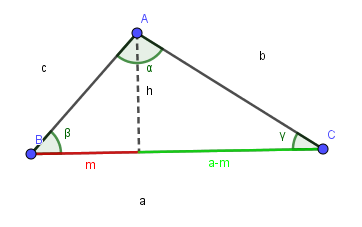
\includegraphics[width=0.50\linewidth]{triangulo.png}
		\end{center}
		\caption{Triângulo para ilustrar a lei dos cossenos.}
		\label{fig:coslaw}
	\end{figure}
	\begin{itemize}
		\item \textbf{Demonstração Leis dos Cossenos:}
		
		Dado um triângulo qualquer, traça-se uma altura relativa ao lado $a$. Aplicando o \textit{Teorema de Pitágoras} no $\Delta ABD$:
		
		\begin{equation}
		c^{2}=m^{2}+h^{2} \rightarrow h^{2}=c^{2}-m^{2}
		\label{eq:tri1}
		\end{equation}
		
		Aplicando novamente \textit{Pitágoras}, porém, em $\Delta ADC$, obtemos:
		\begin{equation}
		b^{2}=h^{2}+(a-m)^{2}
		\label{eq:tri2}
		\end{equation}
		Substituindo na equação ~\ref{eq:tri2} o valor de $h^{2}$ obtido em ~\ref{eq:tri1}:
		$$
		b^{2}=c^{2}-m^{2}+a^{2}-2am+m^{2}
		$$
		$$
		b^{2}=c^{2}+a^{2}-2am
		$$
		Analisando a 
		Figura ~\ref{fig:coslaw}, pode-se perceber que $\frac{m}{c}=\cos\beta$, então:
		$$
		b^{2}=c^{2}+a^{2}-2ac\cos\beta
		$$
		Analogamente, obtém-se:
		$$
		c^{2}=a^{2}+b^{2}-2ab\cos\gamma
		$$
		$$
		a^{2}=b^{2}+c^{2}-2bc\cos\alpha
		$$
		Note também que se o argumento dos cossenos for $\frac{\pi}{2}$ recaímos no Teorema de Pitágoras. $\hfill\blacksquare$
		\item \textbf{Ângulos Entre 2 Vetores:}
		
		Sejam dois vetores $\overrightarrow{u}$ e $\overrightarrow{v} \in \mathbb{R}^2$, representados na Figura ~\ref{fig:diffbtvet}
		\begin{figure}[H]
			\begin{center}
				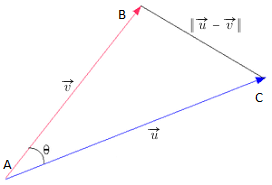
\includegraphics[width=0.4\linewidth]{Angulovetoresnovo.png}
			\end{center}
			\caption{Diferença entre vetores u e v}
			\label{fig:diffbtvet}
		\end{figure}
		Para encontrarmos o angulo $\theta$ utilizaremos a lei dos cossenos aplicada a $\Delta ABC$:
		\begin{equation}
		\|\overrightarrow{u}-\overrightarrow{v}\|^{2}=\|\overrightarrow{u}\|^{2} + \|\overrightarrow{v}\|^{2} - 2\|\overrightarrow{u}\|\|\overrightarrow{v}\|\cos\theta
		\label{eq:ang1}
		\end{equation}
		Utilizando a definição do produto escalar \cite{GASteinbruch}
		\begin{equation}
		\|\overrightarrow{u}-\overrightarrow{v}\|^{2}=\|\overrightarrow{u}\|^{2} + \|\overrightarrow{v}\|^{2} - 2\overrightarrow{u}\overrightarrow{v}
		\label{eq:ang2}
		\end{equation}
		Comparando a equação ~\ref{eq:ang1} com a ~\ref{eq:ang2}, obtemos trivialmente
		$$
		\|\overrightarrow{u}\|^{2} + \|\overrightarrow{v}\|^{2} - 2\|\overrightarrow{u}\|\|\overrightarrow{v}\|\cos\theta = \|\overrightarrow{u}\|^{2} + \|\overrightarrow{v}\|^{2} - 2\overrightarrow{u}\overrightarrow{v}
		$$
		$$
		\overrightarrow{u}\overrightarrow{v} = \|\overrightarrow{u}\|\|\overrightarrow{v}\|\cos\theta
		$$
		Logo,
		$$
		\cos\theta = \frac{\overrightarrow{u}\overrightarrow{v}}{\|\overrightarrow{u}\|\|\overrightarrow{v}\|} 
		$$
		$\hfill\blacksquare$
	\end{itemize}
	
	\newpage
	\phantomsection
	\addcontentsline{toc}{section}{Apêndice B - Matrizes como Transformações Lineares e Sobre $B_i$}
	\section*{Apêndice B} 
	\subsection*{Matrizes como Transformações Lineares e Sobre $B_i$}
	
	Quando se começa a aprender sobre matrizes, no ensino médio, normalmente este é um assunto que lhe é apresentado como algo que caiu do céu, difícil de engolir. Na verdade, não é raro um graduando de matemática ter dificuldades para entende-las.
	
	\subsubsection*{Matrizes}
	
	Uma matriz real $\mathbf{a} = [a_{ij}]$ de dimensões $m \times n$ é definida como uma lista de números $a_{ij}$, onde $i \mid 1 < i < m$ e $j \mid 1 < j < n$ são os índices que, juntos, identificam unicamente cada elemento. Costuma-se representar a matriz $\mathbf{a}$ como um quadro de $m\cdot n$ elementos, onde $m$ é o número de linhas e $n$ é o número de colunas, de forma que o elemento $a_{ij}$ situa-se no cruzamento entre a $i$-ésima linha e a $j$-ésima coluna, como segue:
	
	\[ \mathbf{a} =
	\begin{blockarray}{cccc}
	\begin{block}{[cccc]}
	a_{11} & a_{12} & \cdots & a_{1n} \\
	a_{21} & a_{22} & \cdots & a_{2n} \\
	\vdots & \vdots & \vdots & \vdots \\
	a_{m1} & a_{m2} & \cdots & a_{mn} \\
	\end{block}
	\end{blockarray}\]
	
	Seja $M(m\times n)$ um conjunto de matrizes de tal forma que todas as matrizes de dimensão $m\times n$ estejam dentro dele. Podemos definir algumas operações neste conjunto. São elas: 
	
	\begin{itemize}
		\item \textbf{Soma de Matrizes:} Sejam duas matrizes $\mathbf{a}, \mathbf{b}$ $\in M(m \times n)$, define-se a soma de $\mathbf{a} = [a_{ij}]$ com $\mathbf{b} = [b_{ij}]$ como $$\mathbf{a} + \mathbf{b} = [a_{ij} + b_{ij}]$$
		
		\item \textbf{Multiplicação por Escalar:} Sejam $\mathbf{a} \in M(m \times n)$ e $\lambda \in \mathbb{R}$ um escalar qualquer, o produto de $\mathbf{a} = [a_{ij}]$ por $\lambda$ é definido como $$\lambda \cdot \mathbf{a} = \lambda [a_{ij}] = [\lambda a_{ij}]$$
	\end{itemize}
	
	Tendo estas duas operações construídas, podemos definir também:
	\begin{itemize}
		\item \textbf{Existência de elemento nulo:} Define-se como \textit{matriz nula} $\mathbf{0} \in M(m \times n)$ a matriz formada exclusivamente por $m\cdot n$ zeros.
		
		\item \textbf{Existência do elemento oposto para adição:} Seja $\mathbf{a} \in M(m \times n)$ uma matriz da forma $\mathbf{a} = [a_{ij}]$, define-se o elemento oposto de $\mathbf{a}$ como $-\mathbf{a} = [-a_{ij}].$
	\end{itemize}

	Tendo tais definições, chegamos em um resultado interessante.
	\\
	
	\textbf{Proposição: }O conjunto $M(m \times n)$ é um espaço vetorial. \cite{AlgebraLinearElon}
	\\ \newline	Para chegar na conclusão acima, basta tomar as definições dadas e perceber que podemos escrever cada linha e coluna de uma matriz como vetores, ou seja, $\forall \mathbf{a} \in M(m \times n)$, $\exists$ um \textit{vetor-linha} $a_i^l = (a_{i1}, a_{i2}, \dots, a_{in})$ e um \textit{vetor-coluna} $a_j^c = (a_{1j}, a_{2j}, \dots, a_{mj})$ que representam a $i$-ésima linha e $j$-ésima coluna de $\mathbf{a}$, respectivamente.
	
	Para que possamos continuar, necessitamos introduzir mais um grande tópico de álgebra linear, as \textit{transformações lineares}.
	\subsubsection*{Transformações Lineares}
	Sejam $E, F$ espaços vetoriais. Uma transformação linear $A: E \longrightarrow F$ é uma correspondência que associa a cada vetor $v \in E$ um vetor $A(v) = A\cdot v = Av \in F$ de modo que valham, para quaisquer $u,v \in E$ e $\alpha \in \mathbb{R}$, as relações:  
	$$A(u + v) = A(u) + A(v),$$
	$$A(\alpha\cdot v) = \alpha Av.$$ 
	
	Denominamos o vetor $A\cdot v$ como imagem (ou transformado) de $v$ pela transformação $A$ \cite{AlgebraLinearElon}. Perceba que transformação linear é uma classificação de um conjunto especial de funções, ou seja, aquelas que respeitam os dois requisitos acima.
	\\ \newline \textbf{Teorema:} Sejam $E, F$ espaços vetoriais e $B$ uma base de $E$. A cada vetor $x \in B$, façamos corresponder (de maneira arbitrária) um vetor $b \in F$. Então existe uma única transformação linear $A: E\longrightarrow F$ tal que $A\cdot x = b$ para cada $x \in B$.
	
	A demonstração deste teorema se encontra em \cite{AlgebraLinearElon}. 
	\\
	
	Graças a este enunciado, para podermos definir uma transformação linear $A: \mathbb{R}^n \longrightarrow \mathbb{R}^m$ basta escolher para cada $j = 1, \dots, n$ um vetor $v_j = (a_{1j}, a_{2j}, \dots, a_{mj}) \in \mathbb{R}^m$ de tal forma que $v_j = A \cdot e_j$ é a imagem do $j$-ésimo vetor da base canônica, $e_j = (0, \dots, 1, \dots, 0)$, pela transformação linear $A$. Logo, fica determinada a imagem $A \cdot v$ de qualquer vetor $v = (x_1, \dots, x_n) \in \mathbb{R}^n$. Com efeito, tem-se $v = x_1e_1 + \cdots + x_ne_n$, por tanto podemos escrever
	
	$$A\cdot v = A (\sum_{j=1}^{n}x_je_j) = \sum_{j=1}^{n}x_jA\cdot e_j = \sum_{j=1}^{n}(a_{1j}x_j, a_{2j}x_j, \dots, a_{mj}x_j)$$
	
	Aplicando então o somatório em cada elemento, obtemos
	
	$$A \cdot v= (\sum_{j=1}^{n}a_{1j}x_j, \sum_{j=1}^{n}a_{2j}x_j, \dots, \sum_{j=1}^{n}a_{mj}x_j)$$
	
	Ou seja, cada componente $\sum_{j=1}^{n}a_{ij}x_j$, onde $i \in \mathbb{N} \mid 1<i<m$, representa a componente imagem de $v$ pela transformação $A$. Podemos chamar cada uma dessas componentes de $y_i$, concluindo que
	
	$$A(x_1, x_2, \dots, x_n) = (y_1, y_2, \dots, y_m)$$
	
	onde
	
	\[
	\begin{blockarray}{ccccccccc}
	\begin{block}{ccccccccc}
	y_1   & = & a_{11}x_1 & + & a_{12}x_2 & + & \cdots & + & a_{1n}x_n \\
	y_2   & = & a_{21}x_1 & + & a_{22}x_2 & + & \cdots & + & a_{2n}x_n \\
    \vdots &  & \vdots    &  & \vdots    &  & \vdots &  & \vdots    \\
	y_m   & = & a_{m1}x_1 & + & a_{m2}x_2 & + & \cdots & + & a_{mn}x_n \\
	\end{block}
	\end{blockarray}
	\] 
	
	Interessante, não? Note: Acaba-se de concluir que uma transformação linear $A: \mathbb{R}^n \longrightarrow \mathbb{R}^m$ pode ser inteiramente representada pela matriz $\mathbf{a} = [a_{ij}] \in M(m \times n)$, onde os vetores-coluna dessa matriz são as imagens $A\cdot e_j$ dos vetores da base canônica de $\mathbb{R}^n$ e os vetores-linha são dados pelas componentes da imagem $A\cdot v$ de um vetor arbitrário $v = (x_1, \dots, x_n) \in \mathbb{R}^n$, que podemos representar por um vetor $w = (y_1, \dots, y_m) \in \mathbb{R}^m$. \cite{AlgebraLinearElon} Diz-se que $\mathbf{a}$ é \textit{matriz da transformação} $A$ relativa as bases canônicas de $\mathbb{R}^n$ e $\mathbb{R}^m$.
	
	\subsubsection*{Operando Matrizes}
	As matrizes como vistas até aqui não apresentam muitas dificuldades, são apenas operações de elemento a elemento, sem grandes complicações. Pode-se até imagina-las apenas como uma metodologia de organizar uma grande quantidade de dados, de forma a expressa-los mais facilmente em um padrão de quadro bidimensional, ou seja, contradizendo os argumentos apresentados na introdução deste apêndice. Nesta seção introduziremos a operação que traz para as matrizes esse ar de mistério, estimulando dúvidas: \textit{O produto de matrizes}.
	\\ \newline \textbf{Definição:} Sejam $\mathbf{a} = [a_{ij}] \in M(m \times n)$ e $\mathbf{b} = [b_{ij}] \in M(n \times p)$ matrizes quaisquer de foma que o número de colunas $n$ da matriz $\mathbf{a}$ seja o mesmo que o número de linhas $n$ da matriz $\mathbf{b}$. O produto de $\mathbf{a}$ por $\mathbf{b}$ (nessa ordem) é definido como $\mathbf{ab} = \mathbf{c} = [c_{ij}] \in M(m \times p)$, onde $c_{ij}$ é o $ij$-ésimo elemento da matriz $\mathbf{c}$ e é dado por
	$$c_{ij} = a_{i1}b_{1j} + a_{i2}b_{2j} + \cdots + a_{in}b_{nj} = \sum_{k = 1}^{n}a_{ik}b_{kj}$$
	
	onde $i, j \in \mathbb{N}$ são tais que $1<i<m$ e $1<j<p$.
	
	Também podemos definir o elemento $c_{ij}$ usando como perspectiva o \textit{produto interno de vetores} \cite{AlgebraLinearElon}, onde $a_i^l$ é o $i$-ésimo vetor-linha de $\mathbf{a}$ e $b_j^c$ é o $j$-ésimo vetor-coluna de $\mathbf{b}$, então 
	$$c_{ij} = \langle a_i^l,b_j^c\rangle = a_{i1}b_{1j} + a_{i2}b_{2j} + \cdots + a_{in}b_{nj}$$
	Resultando em 
	
	\[\mathbf{c} =
	\begin{blockarray}{cccc}
	\begin{block}{[cccc]}
	\langle a_1^l,b_1^c\rangle & \langle a_1^l,b_2^c\rangle & \cdots & \langle a_1^l,b_p^c\rangle \\
	\langle a_2^l,b_1^c\rangle & \langle a_2^l,b_2^c\rangle & \cdots & \langle a_2^l,b_p^c\rangle \\
	\vdots & \vdots & \vdots & \vdots \\
	\langle a_m^l,b_1^c\rangle & \langle a_m^l,b_2^c\rangle & \cdots & \langle a_m^l,b_p^c\rangle \\
	\end{block}
	\end{blockarray}\]
	
	Perceba que o produto de matrizes, no geral, não é comutativo, ou seja, $\mathbf{ab} \neq \mathbf{ba}$, salvo exceções, e aqui está o problema no seu estudo. Não é fácil digerir a ideia de um produto não comutativo, ainda mais sem entender de onde ele vem. 	Neste terreno não há intuição geométrica que ajude e nem tente extrapolar este conceito para a dimensão infinita, caso contrário perderá agradáveis noites de sono.
	
	Mas nem tudo está perdido, existem algumas aplicações que nos ajudam a entender melhor esta poderosa ferramenta, como segue.
	\\ \newline \textbf{Exemplo: }Suponha uma transformação linear $A: \mathbb{R}^n \longrightarrow \mathbb{R}^m$, sabemos que esta transformação pode ser inteiramente representada por uma matriz $\mathbf{a} = [a_{ij}] \in M(m\times n)$, conforme visto na seção anterior, logo, a equação $Ax = b$ pode ser inteiramente representada como o produto de matrizes $\mathbf{a} \mathbf{x} = \mathbf{b}$, onde os vetores $x = (x_1, \dots, x_n) \in \mathbb{R}^n$ e $b = (b_1, \dots, b_m) \in \mathbb{R}^m$ passam a ser considerados como matrizes $n\times 1$ e $m\times 1$, respectivamente, ou seja, como vetores-coluna, logo
	
	\[ 
	\begin{blockarray}{cccc}
	\begin{block}{[cccc]}
	a_{11} & a_{12} & \cdots & a_{1n} \\
	a_{21} & a_{22} & \cdots & a_{2n} \\
	\vdots & \vdots & \vdots & \vdots \\
	a_{m1} & a_{m2} & \cdots & a_{mn} \\
	\end{block}
	\end{blockarray}
	\begin{blockarray}{c}
	\begin{block}{[c]}
	x_1 \\
	x_2 \\
	\vdots \\
	x_n \\
	\end{block}
	\end{blockarray}=
	\begin{blockarray}{c}
	\begin{block}{[c]}
	b_1 \\
	b_2 \\
	\vdots \\
	b_n \\
	\end{block}
	\end{blockarray}
	\]
	
	Com isso concluí-se que podemos aplicar algumas funções especiais, as quais respeitam os dois requisitos que definem transformações lineares, utilizando matrizes. Isso se torna deveras interessante quando se necessita resolver problemas de forma computacional que utilizem transformações lineares, pois a utilização de matrizes traz ganhos computacionais significativos \cite{AlgebraLinearElon}. 
	\\
	
	Outra aplicação que demonstra a verdadeira importância da utilização das matrizes é quando necessita-se concatenar transformações lineares, ou seja compor funções.
	\\ \newline \textbf{Definição:} Dadas as transformações lineares $A: E \longrightarrow F$, $B: F \longrightarrow G$, onde o domínio de $B$ coincide com a imagem de $A$, define-se o \textit{produto} $BA: E \longrightarrow G$ colocando, $\forall v \in E$, $(BA)v = B(Av)$, como representado na Figura ~\ref{fig:compfunc}.
	
	\begin{figure}[H]
		\begin{center}
			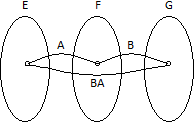
\includegraphics[width=0.4\linewidth]{compfunc.png}
		\end{center}
		\caption{Transformação linear composta BA}
		\label{fig:compfunc}
	\end{figure}
	
	Assim, podemos enunciar o seguinte teorema.
	\\ \newline \textbf{Teorema:} Sejam $A: E \longrightarrow F$ e $B: F \longrightarrow G$, $U = \{u_1, \dots, u_p\} \subset E$, $V = \{v_1, \dots, v_n\} \subset F$ e $W = \{w_1, \dots, w_m\} \subset G$ tal que $\mathbf{a} \in M(m\times p)$ é a matriz de $A$ nas bases $U, V$ e $\mathbf{b} \in M(m\times n)$ é a matriz de $B$ nas bases $V, W$, então a matriz de $BA: E\longrightarrow G$ nas bases $U, W$ é o produto $\mathbf{ba} \in M(m\times p)$ das matrizes $\mathbf{b}$ e $\mathbf{a}$. \cite{AlgebraLinearElon}
	\\
	
	Ou seja, se tivermos duas transformações lineares $A: E \longrightarrow F$ e $B: F \longrightarrow G$, podemos multiplicar suas representações matriciais $\mathbf{b}$ e $\mathbf{a}$ afim de obter o equivalente matricial da função composta $BA: E \longrightarrow G$. Este teorema é muito importante, podendo simplificar um algorítimo de $n$ operações lineares $\mathbf{a_i} \mid 1<i<n$ em apenas uma aplicação da forma $\mathbf{a_{r}x} = \mathbf{b}$, onde $\mathbf{a_{r}}$ é a matriz resultante de $\prod_{i=1}^{n}\mathbf{a}_i$.
	\\
	
	Assim concluímos o estudo sobre transformações lineares e suas representações como matrizes. Podemos aplicar estes conhecimentos em um caso específico de forte interesse neste documento, a matriz $B_i$.
	
	\subsubsection*{Sobre a Matriz $B_i$}
	
	Ao trabalhar-se com dados vindos de experimentos de RMN, é fácil perceber que o sistema de coordenadas cartesianas não é a melhor forma para representar estes dados, pois não se sabe de antemão qual a posição de cada átomo estudado. Como alternativa, utiliza-se as coordenadas internas que, de forma muito semelhante ao sistema de coordenadas esféricas (normalmente visto em calculo no $\mathbb{R}^3$), faz uso de distâncias e ângulos para representar localizações. 
	
	Infelizmente temos um problema: as coordenadas internas não são muito agradáveis. Necessitam de constantes manipulações trigonométricas e possuem complicada interpretação geométrica, pois não dependem de um referencial fixo, ou seja, esse sistema de coordenadas não possui uma origem bem definida como em um plano cartesiano., diferentemente, nesse sistema a referencia se dá sempre partindo da localização atual. Pode-se dizer que a referência é sempre de dentro para fora. Talvez seja daí que venha o termo "coordenadas \textit{internas}", pois o referencial é o interior do ponto que se estuda. 
	
	 Dados os motivos citados, salvo a liberdade poética do autor, temos forte interesse de apresentar os resultados finais de um experimento de RMN em coordenadas cartesianas, ou seja, deve-se transformar coordenadas internas em cartesianas. Infelizmente isso não é uma tarefa fácil e depende muito da configuração espacial que compõe a molécula estudada. Pode-se dizer que o PGDM resume-se nesta transformação de coordenadas. Perceba a importância de se estudar a matriz que possui este papel, no caso, a $B_i$.
	 
	 Conforme apresentado na seção ~\ref{sec:bi}, a $B_i$ é a $i$-ésima matriz $4\times 4$ em um produtório de $i$ matrizes $4\times 4$ que, multiplicadas pelo vetor-coluna $(0,0,0,1)$ dão origem a realização do $i$-ésimo átomo $x_i$ da molécula estudada. Ou seja, 
	 $$ B_i \in M(4\times 4) \mid
	 B_{1}B_{2}\cdots B_{i}\begin{bmatrix}
	 0\\ 
	 0\\ 
	 0\\ 
	 1
	 \end{bmatrix}
	 = \begin{bmatrix}
	 x_{i1}\\ 
	 x_{i2}\\ 
	 x_{i3}\\ 
	 1
	 \end{bmatrix}
	 \:\forall\:  1< i < N,
	 $$
	 
	 onde $N$ é o número de átomos na molécula e o vetor-coluna $(x_{i1}, x_{i2}, x_{i3}, 1)$ é a realização do $i$-ésimo átomo da molécula, ou seja, tal vetor possui componentes que coincidem com as coordenadas do ponto onde está localizado tal átomo no $\mathbb{R}^3$.
	 
	 Como dito anteriormente, o produto de matrizes é uma forma eficiente de concatenar funções e sabemos também que cada matriz $B_i$, necessária para encontrar a $i$-ésima realização na molécula, pode ser vista como representação de uma transformação linear, ou seja, cada $B_i$ pode ser vista como a matriz que compõe todas as operações necessárias para passar da $x_{i-1}$ até a $x_i$ realização, logo
	 $$
	 (B_1 B_2 \cdots B_{i-1})
	 B_i
	 \begin{bmatrix}
	 0\\ 
	 0\\ 
	 0\\ 
	 1
	 \end{bmatrix}
	 = \begin{bmatrix}
	 x_{i1}\\ 
	 x_{i2}\\ 
	 x_{i3}\\ 
	 1
	 \end{bmatrix},
	 $$
	 onde $(B_1,B_2,\cdots,B_{i-1})$ é a matriz que representa todas as operações necessárias para chegar da $x_1$ até a $x_{i-1}$. Perceba que é como se caminhássemos pelas realizações das moléculas, onde sabemos exatamente para onde apontar (pelos ângulos $\theta$ e $\omega$) e exatamente o quanto caminhar (a distância $d$) para ir de uma molécula a outra.
	 
	 Logo, sabemos que a $B_i$ será composta por movimentos de translações e rotações, nos bastando descobrir quais para entende-la. Nos será útil definir estes dois tipos de transformações lineares, como segue:
	 \begin{itemize}
	 	\item \textbf{Translação:} Podemos resumir esta operação em um deslocamento.
	 	
	 	Seja o vetor $v = (a) \in \mathbb{R}$. Perceba que há uma relação biunívoca entre o espaço vetorial $\mathbb{R}$ e o conjunto $C$ de pontos na reta real, ou seja, $\forall \: v \in \mathbb{R} \:\exists! \: u \in C \mid v\equiv u$, logo, podemos movimentar o vetor $v$ de forma a fazer o ponto por ele representado na reta também se movimentar.
	 	
	 	Como faremos isso? É intuitivo imaginar que a solução seja uma função do tipo $f: \mathbb{R} \longrightarrow \mathbb{R} \mid f(x) = (x + 1)$, ou seja, uma função que leva um ponto $x$ para uma unidade mais longe da origem. Infelizmente isso não se trata de uma movimentação, mas sim de um teleporte. Veja, o ponto mudou de lugar instantaneamente! Isso fere a linearidade:
	 	$$f(x+a) = x+a+1 \neq f(x)+f(a) = x+a+2$$ 
	 	
	 	Isso se deve pois quando algo é deslocado ele possui uma velocidade $\frac{\partial}{\partial t}$ associada, ou seja, precisamos deslocá-lo em relação a alguma dimensão específica do espaço vetorial (no caso $t$), logo, precisamos incrementar uma dimensão ao universo de nossa reta para encontrar a transformação linear que desloca um elemento $v$ por ela.
	 	
	 	Fazemos então 
	 	$$f: \mathbb{R}^2 \longrightarrow \mathbb{R} \mid f(x,t) = x+t,$$
	 	ou seja, agora o ponto $x$ ficará uma unidade mais distante da origem assim que a dimensão $t$ também o ficar. Perceba que agora $x$ movimenta-se a medida que $t$ movimenta, sem saltos, logo, respeitando a linearidade
	 	$$f((x,t)+(a,a)) = f(x+a, t+a) = x+t+a+a = f(x,t)+f(a,a).$$
	 	
	 	Como toda transformação linear pode ser escrita como uma matriz, segue que se
	 	$$
	 	f(x,t) = 
	 	\begin{bmatrix}
	 	1 & 1\\
	 	\end{bmatrix}
	 	\begin{bmatrix}
	 	x\\
	 	t
	 	\end{bmatrix}
	 	=
	 	\begin{bmatrix}
	 	x+t
	 	\end{bmatrix}
	 	= x+t
	 	$$
	 	então $\begin{bmatrix} 1 & 1 \end{bmatrix}$ é a matriz que representa tal transformação, nossa translação.
	 	
	 	%preciso falar sobre aquela algebra que almenta uma dimensão na matriz.. esqueci o nome dela :/ Não posso falar nada sem saber o nome :/
	 	
	 	\item \textbf{Rotação:} Quando se quer rotacionar um objeto, sem alterar o formato dele, normalmente recorremos a matrizes de rotação.
	 	
	 	Tentemos definir um operador que rotacione um vetor em um ângulo $\theta$  em torno da origem \cite{AlgebraLinearElon}, ou seja, precisamos de uma transformação linear $R: \mathbb{R}^2 \longrightarrow \mathbb{R}^2$ que, dado um vetor $v = (x,y) \in \mathbb{R}^2$, seja $Rv = (x', y')$. Como
	 	$$
	 	Rv = 
	 	\begin{bmatrix}
	 	a & b\\
	 	c & d
	 	\end{bmatrix}
	 	\begin{bmatrix}
	 	x\\
	 	y
	 	\end{bmatrix}
	 	=
	 	\begin{bmatrix}
	 	x'\\
	 	y'
	 	\end{bmatrix},
	 	$$
		então $x' = ax + by$ e $y' = cx + dy$. 
		
		Perceba que nosso objetivo é encontrar $a,b,c$ e $d$.
		Sabemos que se $B_{\mathbb{R}^2} = \{(1,0),(0,1)\}$ é a base canônica do $\mathbb{R}^2$, então $R(1,0) = (a,c)$ e $R(0,1) = (b,d)$. Por construção, se rotacionarmos os versores $(1,0)$ e $(0,1)$ em um ângulo $\theta$, conforme Figura ~\ref{fig:rota}, seguindo as definições de senos e cossenos, obtemos que $R(1,0) = (cos(\theta), sen(\theta))$ e $R(0,1) = (-sen(\theta), cos(\theta))$.
		
		\begin{figure}[H]
			\begin{center}
				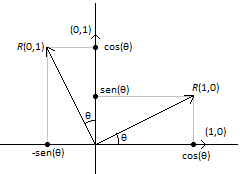
\includegraphics[width=0.5\linewidth]{rota.png}
			\end{center}
			\caption{Transformação linear composta BA}
			\label{fig:rota}
		\end{figure}
	 
	 	Logo, $x' = x cos(\theta) - y sen(\theta)$ e $y' = x sen(\theta) + y cos(\theta)$. Nossa matriz de rotação em torno da origem fica:
	 	$$
	 	\begin{bmatrix}
	 		a & b\\
	 		c & d
	 	\end{bmatrix}
	 	=
	 	\begin{bmatrix}
	 	cos(\theta) & -sen(\theta)\\
	 	sen(\theta) & cos(\theta)
	 	\end{bmatrix}.
	 	$$
	 	
	 	Podemos enxergar esta rotação como uma projeção de uma transformação no espaço tridimensional $\mathbb{R}^3$, onde a rotação acontece ao redor do eixo $z$ (que sai do papel), mantendo o eixo fixo. Para tentarmos ampliar esta matriz para a terceira dimensão, basta que nós entendamos que as componentes da transformação devem ser tais que não modifiquem componentes no eixo z, logo:
	 	$$
	 	\begin{bmatrix}
	 	cos(\theta) & -sen(\theta)\\
	 	sen(\theta) & cos(\theta)
	 	\end{bmatrix}
	 	\begin{bmatrix}
	 	x\\
	 	y
	 	\end{bmatrix}
	 	=
	 	\begin{bmatrix}
	 	x'\\
	 	y'
	 	\end{bmatrix}
	 	\longrightarrow
	 	\begin{bmatrix}
	 	cos(\theta) & -sen(\theta)&0\\
	 	sen(\theta) & cos(\theta)&0\\
	 	0 & 0 & 1
	 	\end{bmatrix}
	 	\begin{bmatrix}
	 	x\\
	 	y\\
	 	z
	 	\end{bmatrix}
	 	=
	 	\begin{bmatrix}
	 	x'\\
	 	y'\\
	 	z'
	 	\end{bmatrix},
	 	$$
	 	
	 	onde $z' = z$.
	 	
	 	A mesma lógica pode ser aplicada para deduzir as rotações em torno dos demais eixos, onde todas são enunciadas a seguir.
	 	
	 	$$
	 	R_x(\theta)\cdot(x,y,z) =
	 	\begin{bmatrix}
	 	1 & 0 & 0\\
	 	0&cos(\theta) & -sen(\theta)\\
	 	0&sen(\theta) & cos(\theta)
	 	\end{bmatrix}
	 	\begin{bmatrix}
	 	x\\
	 	y\\
	 	z
	 	\end{bmatrix}
	 	=
	 	\begin{bmatrix}
	 	x'\\
	 	y'\\
	 	z'
	 	\end{bmatrix},
	 	$$
	 	
	 	$$
	 	R_y(\theta)\cdot(x,y,z) =
	 	\begin{bmatrix}
	 	cos(\theta)&0 & -sen(\theta)\\
	 	0 & 1 & 0\\
	 	sen(\theta) & 0&cos(\theta)
	 	\end{bmatrix}
	 	\begin{bmatrix}
	 	x\\
	 	y\\
	 	z
	 	\end{bmatrix}
	 	=
	 	\begin{bmatrix}
	 	x'\\
	 	y'\\
	 	z'
	 	\end{bmatrix}.
	 	$$
	 	
	 	$$
	 	R_z(\theta)\cdot(x,y,z) =
	 	\begin{bmatrix}
	 	cos(\theta) & -sen(\theta)&0\\
	 	sen(\theta) & cos(\theta)&0\\
	 	0 & 0 & 1
	 	\end{bmatrix}
	 	\begin{bmatrix}
	 	x\\
	 	y\\
	 	z
	 	\end{bmatrix}
	 	=
	 	\begin{bmatrix}
	 	x'\\
	 	y'\\
	 	z'
	 	\end{bmatrix},
	 	$$
	 \end{itemize}	
 
 \newpage
 	Agora que possuímos tais definições, podemos voltar a analisar nossa $B_i$. Então, anunciando-a, sendo $i=4, \dots, N$:
 	$$
 	B_i\:=\:{
 		\begin{bmatrix}
 		-\cos(\theta_{i-2,i}) & -\sin(\theta_{i-2,i}) & 0 & -d_{i-1,i}\cos(\theta_{i-2,i})\\ 
 		\sin(\theta_{i-2,i})\cos(\omega_{i-3,i}) & -\cos(\theta_{i-2,i})\cos(\omega_{i-3,i})
 		& -\sin(\omega_{i-3,i}) & d_{i-1,i}\sin(\theta_{i-2,i})\cos(\omega_{i-3,i})\\ 
 		\sin(\theta_{i-2,i})\sin(\omega_{i-3,i}) & -\cos(\theta_{i-2,i})\sin(\omega_{i-3,i}) & \cos(\omega_{i-3,i}) & d_{i-1,i}\sin(\theta_{i-2,i})\sin(\omega_{i-3,i})\\ 
 		0 & 0 & 0 & 1
 		\end{bmatrix},}
 	$$
 	
 	Pode-se deduzir, decompondo esta matriz em tentativas de composições com as matrizes de translação e rotações descritas, que esta matriz trata-se de 
 	$$
 	B_i=R_{x}(w_{i-3,i}).R_{x}(\pi).R_{z}(\theta_{i-2,i}).R_{y}(\pi).T_{x}(d_{i-1,i}),
 	$$
 	
 	onde, perceba, as operações são compostas da direita para a esquerda, ou seja, primeiro há uma translação e depois um conjunto de quatro rotações. Dentre essas, duas são de um angulo fixo $\pi$, isto se deve ao fato de que, como estamos caminhando de um átomo a outro, toda vez que chegamos em um novo átomo deve-se primeiro olhar para trás (para o átomo anterior) e só então definir aonde está a próxima direção à se percorrer, pois os ângulos assim são definidos (vide Figura ~\ref{fig:angulos}).
 	
\end{document}